%% Kelp Forest Collapse & Recovery -- CS 4632 Project Proposal
%% ACM article class, non-conference (nonacm) two-column conference style.
\documentclass[manuscript,nonacm,11pt]{acmart}

\AtBeginDocument{%
  \providecommand\BibTeX{{%
    Bib\TeX}}}

\settopmatter{printacmref=false}
\renewcommand\footnotetextcopyrightpermission[1]{}
\authorsaddresses{}  % suppress the first-page footer address block

\usepackage{booktabs}
\usepackage{graphicx}
\usepackage{tabularx}
\usepackage{float}

% No paragraph indentation; separate paragraphs with vertical space instead.
\AtBeginDocument{%
  \setlength{\parindent}{0pt}%
  \setlength{\parskip}{0.6em plus 2pt minus 1pt}%
}

\begin{document}

\title{Restoring Our Kelp Forests: A Multi-Trophic\\ Coastal Ecosystem Simulator}

\author{Bryan Agamu}
\affiliation{%
  \institution{Kennesaw State University, CS 4632: Modeling and Simulation}
  \country{USA}
}
\email{}

\renewcommand{\shortauthors}{Bryan}

\begin{abstract}
Wild Kelp forests have been observed to abruptly flip from a lush garden into low diversity
barren landscapes typically referred to as ``urchin deserts''. This happens when their key grazer,
the sea urchin, loses its keystone predator the sea otter.
This paper describes an agent-based simulation of a three-level trophic system (kelp, sea urchins, sea
otters) on a two-dimensional spatial grid. The simulation will be implemented in Python
and will track seven quantitative metrics across seeded Monte~Carlo runs.
\end{abstract}

\maketitle
\pagestyle{plain}  % page numbers only; no title/author running header
\thispagestyle{plain}

%% ============================================================
\section{Project Overview}

\textbf{Project Title:} Understanding Kelp Forest Collapse \& Recovery: A Coastal Ecosystem Simulator.

\textbf{Domain:} Marine ecology and population dynamics. 

\subsection{Problem Statement}
Kelp forests can exist in two different states: a lush healthy canopy that supports high biodiversity,
or a reduced ``urchin barren'' where sea urchins have stripped all of the rocks bare.
My simulation is designed to answer:
\begin{itemize}
  \item At what sea-otter mortality rate does the system collapse into a barren?
  \item Is collapse reversible by simply restoring otters, or does recovery require
        more work than the disturbance that triggered collapse?
  \item How does the spatial clustering of urchins change outcomes, and what is the most effective
        method of recovery?
\end{itemize}

\subsection{Scope}
\textbf{Will simulate:} Three trophic levels as discrete agents/resources on a
grid, spatial foraging, movement, reproduction, and death, stochastic
disturbances (storms, disease). 

\textbf{Will not simulate:} The full marine food cycle (plankton, fish,
invertebrate diversity). Ocean chemistry, currents, or fluid dynamics, genetic or evolutionary adaptation, and
real geographic coastlines (an abstract rectangular grid is used).

%% ============================================================
\section{System Description}

\subsection{System Components}

\begin{table}[H]
  \caption{Core entities, their state, and behaviors.}
  \label{tab:components}
  \small
  \begin{tabularx}{\linewidth}{@{}>{\raggedright\arraybackslash}p{2.4cm}XX@{}}
    \toprule
    \textbf{Entity} & \textbf{Key properties} & \textbf{Behaviors} \\
    \midrule
    Kelp (resource) & biomass, growth rate, max density &
      They regrow or are consumed by urchins \\
    Sea urchin (eats Kelp) & position, energy, age, reproduction threshold &
      They graze, move, reproduce, flee, die / be eaten \\
    Sea otter (eats Urchin) & position, energy, hunger, age &
      They hunt urchins, raft, reproduce, starve and die \\
    Grid cell (rocks that grow Kelp) & substrate, temperature, disturbance state &
      It hosts kelp and propagates storm events \\
    \bottomrule
  \end{tabularx}
\end{table}

\subsection{System Dynamics}
Components interact across all three trophic levels every time step:
\begin{itemize}
  \item \textbf{Top-down control:} otters eat urchins, suppressing the
        herbivore population. Less urchins means more kelp growth
  \item \textbf{Bottom-up limitation:} local kelp density bounds urchin energy
        intake and reproduction. Less kelp density means urchins can intake and reproduce more effectively
  \item \textbf{Collapse cascade:} removing otters lets urchins explode, kelp is
        grazed away, a barren forms, urchins then starve, the system settles
        into a low-biomass ``urchin desert'' stable state.
  \item \textbf{Spatial coupling:} local depletion forces movement, producing
        emergent urchin grazing fronts, otter rafts, and kelp refuges that a
        non-spatial model would not capture.
  \item \textbf{Stochastic disturbance:} random storms and disease arrive as
        events that kill predators and hence, reset kelp patches. They may locally and temporarily 
        rescue or doom populations.
\end{itemize}

\subsection{Core Models and Algorithms}
\label{sec:models}

\paragraph{(1) Lotka--Volterra dynamics with carrying capacity.}
The classical predator--prey system~\cite{lotka1925,volterra1926} provides the
baseline rate structure. In continuous form with logistic prey growth,
\begin{align}
  \frac{dN}{dt} &= rN\!\left(1-\frac{N}{K}\right) - f(N)\,P, \\
  \frac{dP}{dt} &= e\,f(N)\,P - mP,
\end{align}
where $N$ is prey (urchin) density, $P$ is predator (otter) density, $r$ the
prey growth rate, $K$ the carrying capacity, $e$ a conversion efficiency, and
$m$ the predator mortality. I reduced these rates into per-step
probabilities that govern reproduction and predation for each agent.
\textit{Equations from:}~\cite{lotka1925, volterra1926}.

\paragraph{(2) Holling Type~II functional response.}
Predation saturates at high prey density because predators need handling time
per kill~\cite{holling1959}:
\begin{equation}
  f(N) = \frac{aN}{1 + a h N},
\end{equation}
with attack rate $a$ and handling time $h$. This sets each otter's per-step
probability of a successful hunt as a function of nearby urchin density.
\textit{Equations from:}~\cite{holling1959}.

\paragraph{(3) Logistic resource regeneration.}
Each cell's kelp biomass $B$ regrows toward a light-limited maximum
$B_{\max}$:
\begin{equation}
  B_{t+1} = B_t + g\,B_t\!\left(1 - \frac{B_t}{B_{\max}}\right) - C_t,
\end{equation}
where $g$ is the growth rate and $C_t$ the biomass grazed that step. This is the
bottom-up bound coupling resources to consumer dynamics.
\textit{Equations from:}~\cite{lotka1925}.

\paragraph{(4) Stochastic event model.}
Reproduction, death, and predation outcomes are Bernoulli draws each tick;
environmental disturbances (storms, disease) arrive as Poisson events with rate
$\lambda$, $P(k \text{ events}) = \lambda^k e^{-\lambda}/k!$. This supplies the
simulation's required randomness and lets us study variance and extinction
frequency across different seeds.
\textit{Equations from:}~\cite{railsback2019}.

\subsection{Assumptions}
The grid is closed, so agents cannot migrate across its boundaries. Kelp is
modeled as continuous blob of biomass per cell rather than individual plants. Each
step is a fixed biological interval, such as one week. Agents of the same type share the same
parameters within a species, which is not true in nature. Otters eat only urchins and urchins
eat only kelp, so each level has a single prey. Disturbances are local and
independent of one another.

%% ============================================================
\section{Implementation Approach}

\textbf{Programming Language.} Python, chosen for rapid
prototyping, readable logic and useful libraries.

\textbf{Environment / Libraries.} \textbf{NumPy} for grid state and vectorized
rate computation, \textbf{Mesa} for agent-based scheduling, \textbf{Matplotlib}
for generating population time series graphs and grid, \& snapshots
\textbf{pandas} for metrics logging and analysis, \textbf{pytest} for
testing, \textbf{Git/GitHub} for version control.

\textbf{Simulation Type.} Agent-based, discrete-time simulation, with
continuous-equation rate models setting individual agent decisions.

\textbf{Data Collection Plan.} The model logs seven metrics: (1)~per-species
population time series (counts and biomass); (2)~kelp coverage percentage over
time; (3)~the tipping-point threshold (otter mortality at collapse);
(4)~the hysteresis gap between collapse and recovery thresholds; (5)~a spatial
clustering index (Moran's~$I$) for urchins; (6)~time-to-recovery under each
intervention; and (7)~ecosystem stability/variance and extinction frequency
across seeded runs.

%% ============================================================
\section{Literature Review}

\paragraph{Lotka (1925)~\cite{lotka1925}.} Establishes the coupled
differential equations of interacting populations.
It provides our baseline predator--prey rate structure. I discretize 
the equations into per-agent, per-step probabilities and add an explicit
carrying-capacity term.

\paragraph{Volterra (1926)~\cite{volterra1926}.} Independently derives
swaying predator--prey dynamics and the conservation laws governing them.
It predicts the population cycles our model should reproduce
before collapse dynamics are introduced. 

% \emph{Adaptation:} used as a validation
% target, the spatial model must recover qualitatively correct oscillations in
% the no-disturbance limit.

\paragraph{Holling (1959)~\cite{holling1959}.} Introduces functional response
types and the handling-time mechanism behind predator saturation.
It governs otter predation rate as a function of urchin
density. The Type~II curve is converted to a per-step hunt
probability bounded by handling time.

\paragraph{Estes \& Palmisano (1974)~\cite{estes1974}.} The seminal empirical
demonstration that sea otters are a keystone predator whose removal triggers
urchin barrens. It justifies the otter as the control variable for collapse, and
I use it to parameterize the collapse cascade and to ground-truth the
qualitative barren-formation behavior.

\paragraph{Scheffer et al.\ (2001)~\cite{scheffer2001}.} A synthesis of
alternative stable states, catastrophic shifts, and hysteresis in ecosystems.
It is the theoretical backbone for our tipping-point and hysteresis questions,
and it informs the experimental design that sweeps mortality up (to find
collapse) and back down (to find recovery), the gap between which quantifies
hysteresis.

\paragraph{Filbee-Dexter \& Scheibling (2014)~\cite{filbeedexter2014}.} A
focused review treating urchin barrens explicitly as an alternative stable state
of collapsed kelp ecosystems, including spatial and feedback mechanisms.
It directly matches our domain and validates the two-state framing, and it
guides parameter ranges and the spatial mechanisms (grazing fronts, refugia)
we implement.

\paragraph{Railsback \& Grimm (2019)~\cite{railsback2019}.} A practical text on
agent-based and individual-based modeling, scheduling, and the ODD protocol.
It provides architectural guidance for the simulation loop and scheduler: our
class structure and per-tick activity flow follow its design patterns, and
results documentation will follow the ODD protocol.

%% ============================================================
\section{System Architecture (UML)}

\subsection{Class Diagram}
Figure~\ref{fig:class} shows the static architecture. An abstract
\texttt{Agent} base class is specialized by \texttt{Urchin} and \texttt{Otter}
via inheritance. \texttt{Kelp} is a resource owned by each \texttt{GridCell};
\texttt{Grid} is composed of cells; and \texttt{Simulation} composes the
\texttt{Grid}, \texttt{Scheduler}, \texttt{DisturbanceModel},
\texttt{DataCollector}, and \texttt{Params}. Dashed dependencies capture the
trophic interactions (otters prey on urchins; urchins graze kelp) and the
observer relationship of the data collector.

\begin{figure}[p]
  \centering
  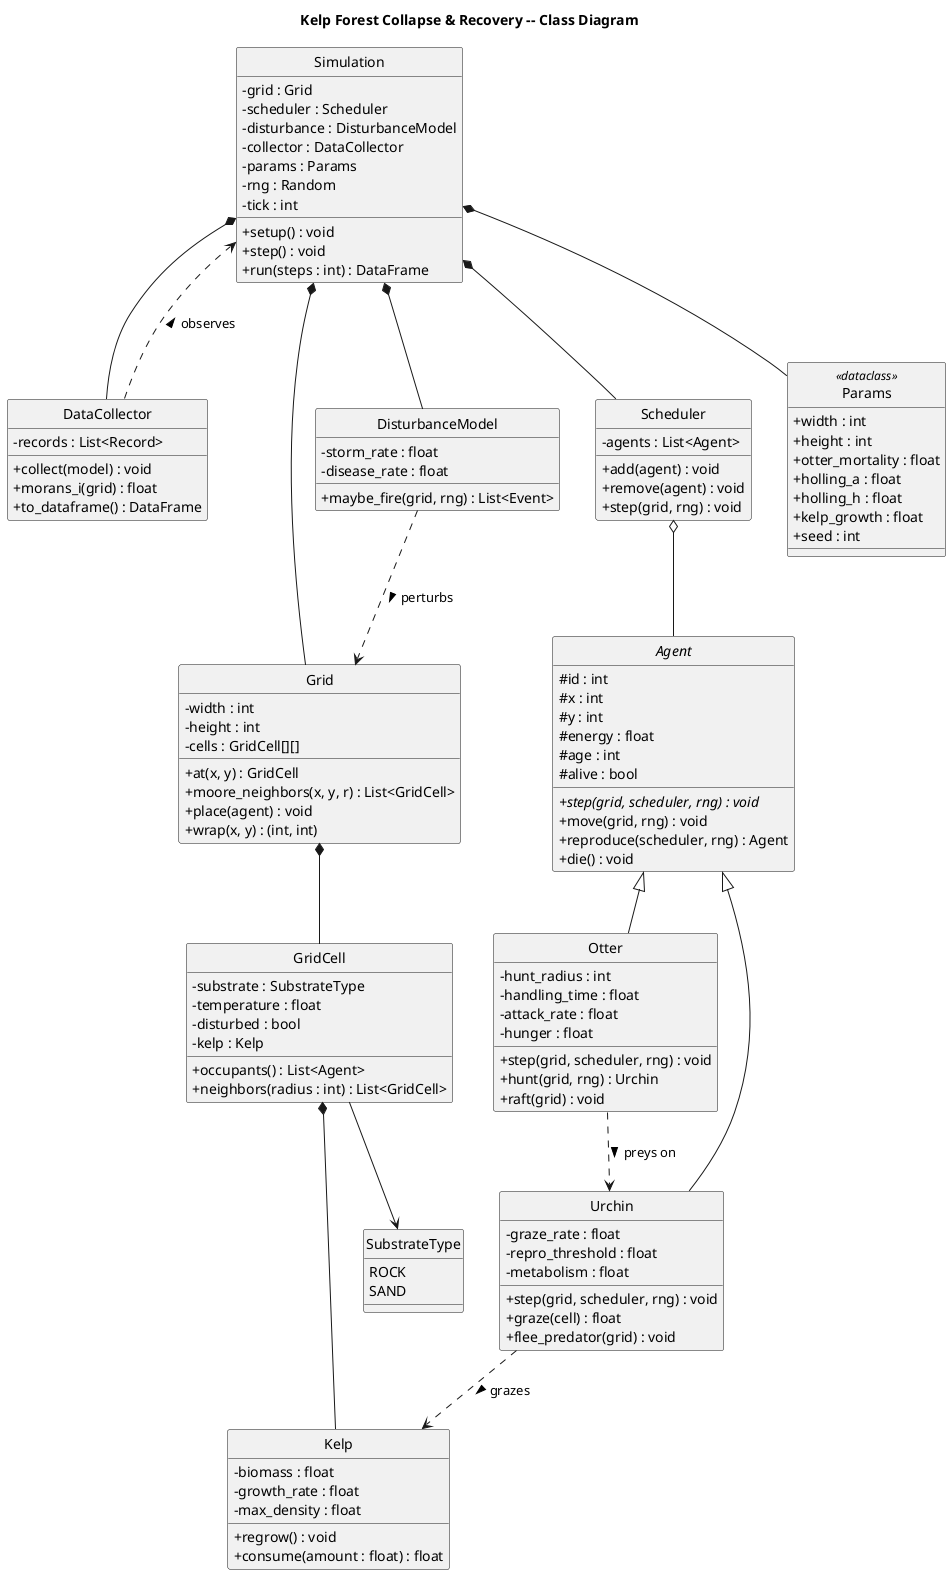
\includegraphics[height=0.9\textheight]{class_diagram.png}
  \caption{Class diagram of the simulation architecture, showing inheritance
  (\texttt{Agent}$\rightarrow$\texttt{Urchin}/\texttt{Otter}) and composition
  (\texttt{Simulation}, \texttt{Grid}, \texttt{GridCell}).}
  \label{fig:class}
\end{figure}

\subsection{Activity Diagram}
Figure~\ref{fig:activity} shows the per-tick control flow of the main simulation
loop. First the kelp regrows. Then the agents are activated in a shuffled order
to sense and act (hunt, flee, move, graze) under their respective models. Next
the model resolves reproduction and death, and fires stochastic disturbance
events. Finally it collects metrics and advances the tick. The loop repeats
until the step limit or extinction is reached.

\begin{figure}[p]
  \centering
  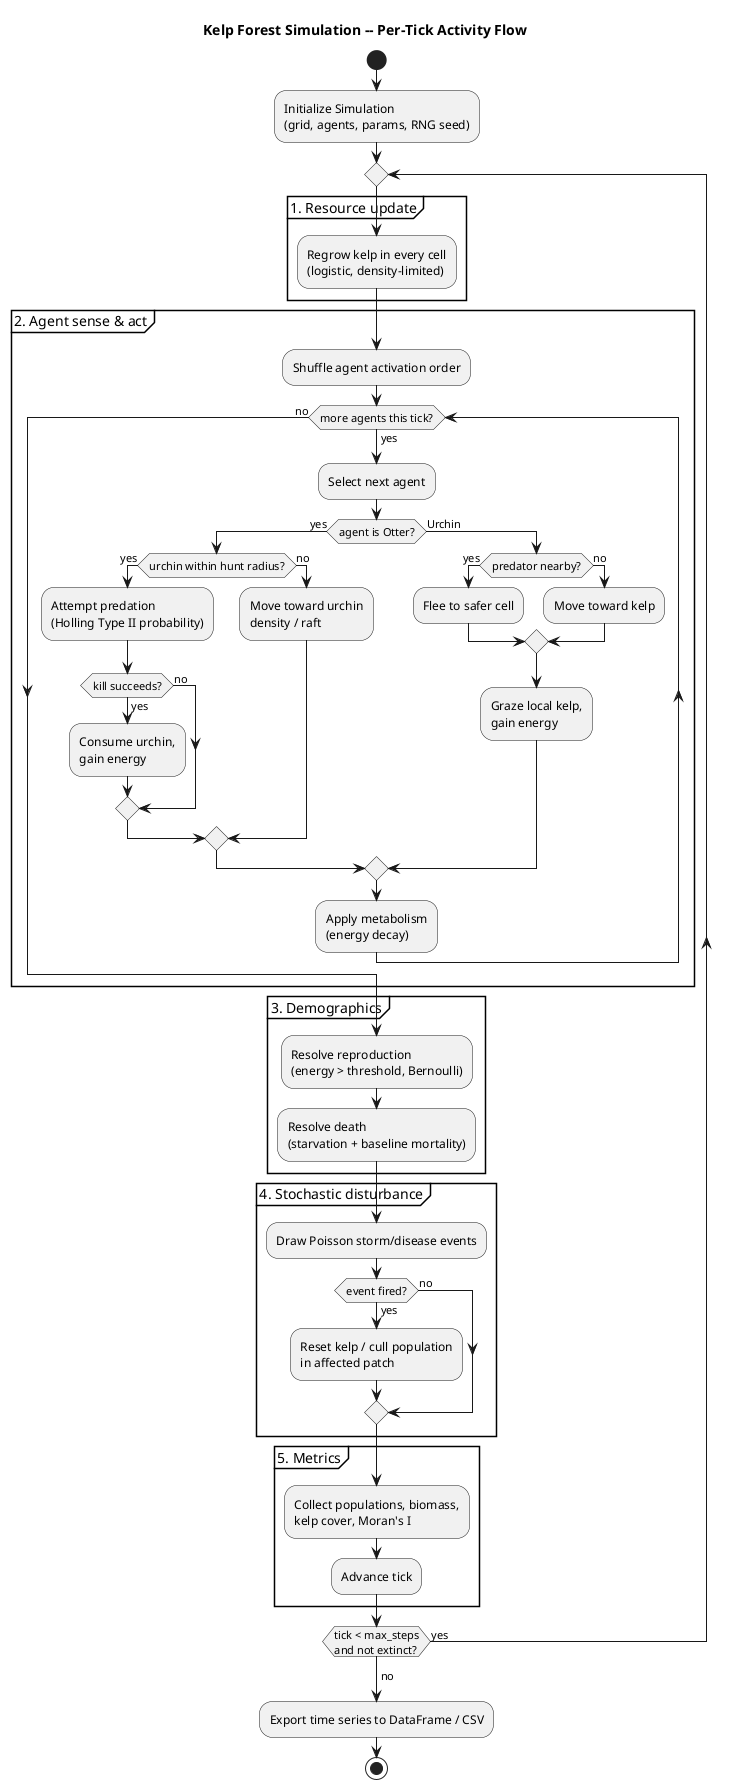
\includegraphics[height=0.9\textheight]{activity_diagram.png}
  \caption{Activity diagram of the per-tick simulation loop.}
  \label{fig:activity}
\end{figure}


\clearpage
\section{Repository}
All code, diagrams, and this document are version-controlled at the project
GitHub repository (https://github.com/jxc2000-b/msim-proj/blob/main/README.md). The initial commit
includes a \texttt{README.md}, the Python project structure, a
Python/\LaTeX{} \texttt{.gitignore}, the UML sources, and this proposal.

\section{Note on AI Use}
An AI assistant was used as a tool during this project to help scaffold and debug the
simulation code, draft and format this \LaTeX{} document from the ACM template, plus help 
generate and clean the PlantUML UML diagrams. All design decisions, model choices, parameters, and the
research questions are my own, and I have reviewed and verified the resulting
code, text, and citations.

%% ============================================================
\bibliographystyle{ACM-Reference-Format}
\bibliography{references}

\end{document}
